\documentclass[12pt, a4paper]{report}
\usepackage[utf8]{inputenc}
\usepackage{caption}

\usepackage{float}

\usepackage{natbib}
\usepackage{graphicx}

\begin{document}

\chapter{Data extractor}
\section{Introduction}
Generally, a search engine has some tasks to do before the user issues
a query. First, the search engine collects pages from the whole Web and
stores them in databases called a repository. This task is called crawling. More concretely, crawling programs follow links from seed pages as special origin pages and visit all the linked pages as destination pages and collect the contents of the pages.\\
So data extraction from the web include some fundamental step:
\begin{enumerate}
    \item Crawling
    \item Ranking
    \item Scraping
\end{enumerate}
\section{Steps}
In this section, we'll describe what each step consists of and  the algorithms used.
\subsection{Crawling Web Pages}
In a word, crawling collects a Web page and its URL (uniform resource
locator), a path to a host name and a file.
\subsubsection{Characteristics}
\begin{itemize}
    \item Robustness:\\
    The Web contains servers that create spider traps, which are generators of web pages that mislead crawlers into getting stuck fetching an infinite number of  pages in a particular domain. Crawlers must be designed to be resilient to such traps. Not all such traps are malicious; some are the inadvertent side effect of faulty website development.
    \item Politeness:\\
    Web servers have both implicit and explicit policies regulating the rate at which a crawler can visit them. These politeness policies must be respected.
    \item Freshness:\\
    In many applications, the crawler should operate in continuous mode: It should obtain fresh copies of previously fetched pages. For such continuous crawling, a crawler should be able to crawl a page with a frequency that approximates the rate of change of that page.
    \item Performance and efficiency:\\
    The crawl system should make efficient use of various system resources including processor, storage, and network bandwidth.
    \item Quality: \\
    Given that a significant fraction of all web pages are of poor utility for serving user query needs, the crawler should be biased toward fetching “useful” pages first.
\end{itemize}

\subsubsection{General Algorithm}
Given a set of URLs (seed) from to start crawling.
\begin{enumerate}
    \item Insert URLs of Web sites as seeds into a data structure called pool (Queue).
    \item Repeat the following steps until no more URLs are found (i.e., the pool is empty)
    \item Delete a URL from the pool.
    \item Visit the page pointed by the URL and collect URLs contained by the page. 
    \item Insert the newly collected URLs into the pool.
    \item Indexing: Extract page information and link information from the accessed page and store the former and the latter in the page repository and the link repository, respectively
\end{enumerate}
This general algorithm doesn't specify how to navigate through the URLs, and which ones to keep since it can't search every possible URL.
\subsubsection{Variants}
\begin{itemize}
    \item BFS (Breadth First Search):\\
        This method differs from the general algorithm in the way it add new URLs (at the rear end of the pool) and retrieves the next URL to process (from the front end of the pool).
    \item DFS (Depth First Search):\\
        This method differs from the general algorithm in the way it add new URLs (at the front end of the pool) and retrieves the next URL to process (from the front end of the pool).
    \item Fish Search:\\
        It takes as input a seed URL and a search query, and dynamically builds a pool (initialized to the seed URL) of the next URLs (hereafter called nodes) to be explored. At each step the first node is popped from the pool and processed. As each document's text becomes available, it is analyzed by a scoring component evaluating whether it is relevant or irrelevant to the search query (\{1,0.5,0\} value) and, based on that score, a heuristic decides whether to pursue the exploration in that direction or not: Whenever a document source is fetched, it is scanned for links. The nodes pointed to by these links (denoted "children") are each assigned a depth value. If the parent is relevant, the depth of the children is set to some predefined value. Otherwise, the depth of the children is set to be one less than the depth of the parent. When the depth reaches zero, the direction is dropped and none of its children is inserted into the list.
        \begin{figure}[H]
           \begin{center}
\makebox[\textwidth][c]{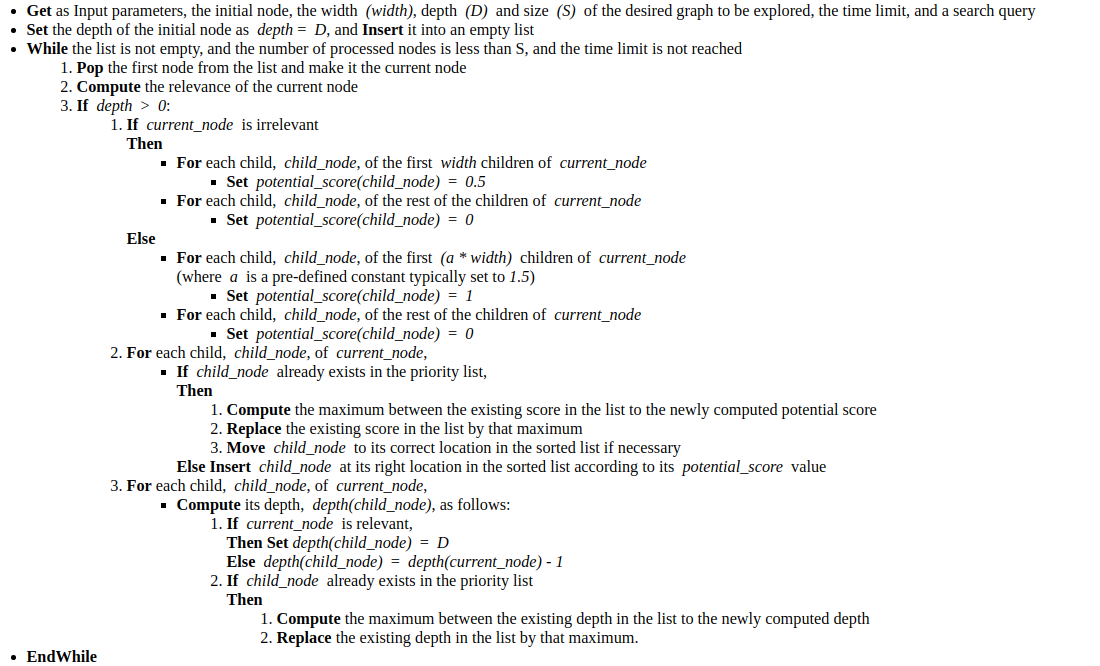
\includegraphics[width=1.5\textwidth]{fish_search.png}}
            \caption{Fish Search Algorithm}
\label{fig:fish_search}
\end{center}
        \end{figure}
        
        

    \item Shark Search Algorithm:\\
        This is a variant of the Fish Search, this one change the way we score each page from \{1,0.5,0\} to a continuous [0,1] based on relevancy of its neighbour nodes using the following algorithm:\\
        \begin{figure}[H]
           \begin{center}
\makebox[\textwidth][c]{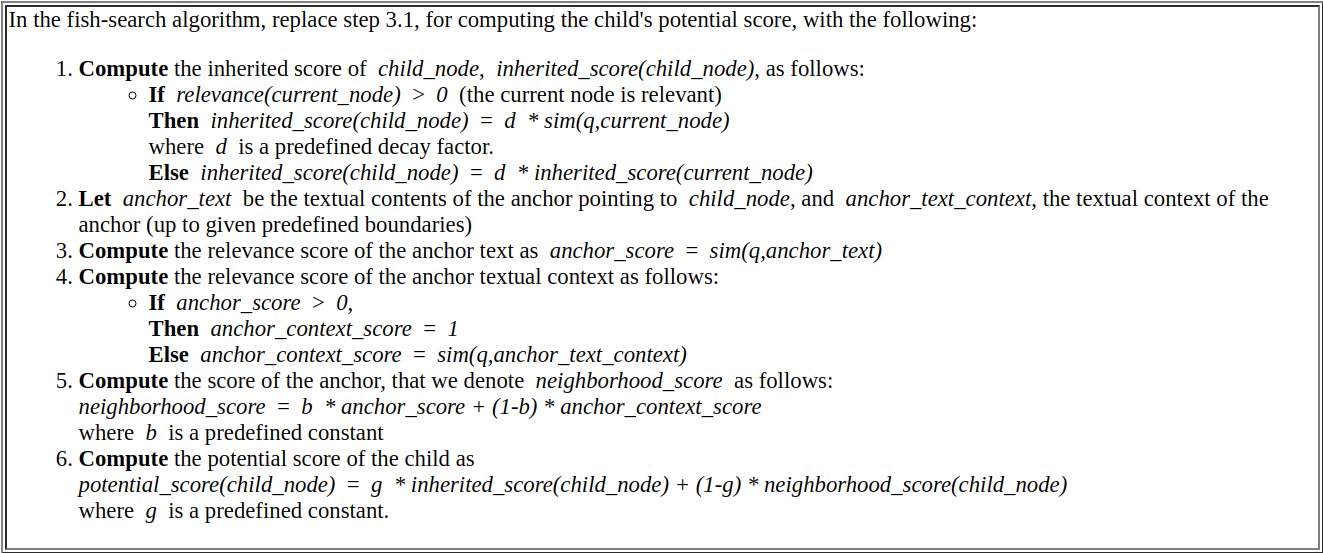
\includegraphics[width=1.5\textwidth]{shark_search.png}}
            \caption{Shark Search Algorithm}
\label{fig:shark_search}
\end{center}
        \end{figure}

    \item Path-Ascending Crawling:\\
        Given a page, the path ascending crawling algorithm would crawl each path from the home to the last file of that URL.\\
        For e.g: URL =http://rashmi.org/rash/profit.html, it will attempt to crawl http://rashmi.org/, http://rashmi.org/rash/ and http://rashmi.org/rash/profit.html.

\end{itemize}

\subsection{Ranking}
Some search engines adopt specific methods (e.g., PageRank of Google) to calculate ranks which express the importance of the crawled pages statistically in advance of search. Other search engines use similar methods (e.g., HITS) to calculate the ranks of pages dynamically; calculate the ranks for all the searched pages by
taking the similarity with search terms into consideration.
\subsubsection{Algorithms}
\begin{itemize}
    \item PageRank:\\
    The PageRank theory holds that an imaginary surfer who is randomly clicking on links will eventually stop clicking.\\
    The rank of a page is defined as the likelihood that a surfer will visit that page from any given page, it is calculated as follows: 
$$PR(p_i,t+1)=\frac{1-d}{N}+d\sum_{p_j\in M(p_i)}\frac{PR(p_j,t)}{L(p_j)}$$
\begin{itemize}
    \item $PR(p_i)$: Page rank of $p_i$
    \item $d$: Dumping factor; The probability, at any step, that the person will continue surfing links that are from the page where he is currently in not exit it and choose a new page randomly from the set of all the pages.
    \item $N$: Maximum number of pages generated by the crawler.
    \item $M(p_i)$: The set of page pointing at the $p_i$
    \item $L(p_j)$: The number of links at the page $p_j$
\end{itemize}
    \item Other Algorithms: OPIC(On-line Page Importance Computation), ,HITS(Hyperlink-Induced Topic Search), Vector Space Model.
\end{itemize}

\subsection{Scraping}
It's the process of retrieving data from a specific page. It can be done by using an API (such in the case of social media websites) or parsing HTML, source code , of the page.
\subsubsection{Wrappers}
 Wrapper defined as an application procedure to extracts content regarding a specific data source, that does not provide any API , or translates the data into a relational form. This task is separated into three sub-tasks:
\begin{enumerate}
    \item Generation:\\
        Can be done using regular expression, DOM Tree (Nodes represent html tags/sections).
    \item Extraction:\\
    Information Extraction operates a task by automatically extracting structured information out of unstructured and/or semi-structured machine-readable documents. This approach activity consists of the processing of human language text by using the natural language processing (NLP).
    \item Maintenance:\\
    The wrapper maintenance arises because the template of the web source may experiment changes that invalidate the current wrappers. 
\end{enumerate}









\section{References:}
\begin{itemize}
    \item Hiroshi Ishikawa - Social big data mining-CRC Press an imprint of Taylor \& Francis Group (2013).
    \item Fish Search: http://www.cs.cmu.edu/~dpelleg/bin/360.html
    \item Analysis of Web Crawling Algorithms, by: Rashmi Janbandhu, Prashant Dahiwale, M.M.Raghuwanshi.
    \item Wrappers : Wrapper approaches for web data extraction : A review.
    \item Wrappers: Analysis Of Different Web Data Extraction Techniques.
    
\end{itemize}

\end{document}
